\subsection{MODFLOW models}
in this section the designed MODFLOW models are tested (see \hyperref[fig_logbook_1.0_CONGROMO]{\textcolor{blue}{Figure }\ref{fig_logbook_1.0_CONGROMO}} for the designed models).  Model 1 shows head values to be symmetrical around the well in the centre of the model as expected (\hyperref[fig_logbook1_top]{\textcolor{blue}{Figure }\ref{fig_logbook1_top}}). For all models a cross sectional view shows similar symmetrical behaviour around the well (\hyperref[fig_logbook1_side]{\textcolor{blue}{Figure }\ref{fig_logbook1_side}}). The well is located in the upper most layer in every model, with a constant pumping rate, one would expect flow paths to be towards the well for all layers. This is indeed the case as can be seen by the deeper layers having increasingly large hydraulic heads (\hyperref[fig_logbook1_side]{\textcolor{blue}{Figure }\ref{fig_logbook1_side}}).

\begin{figure}[ht]
\centering
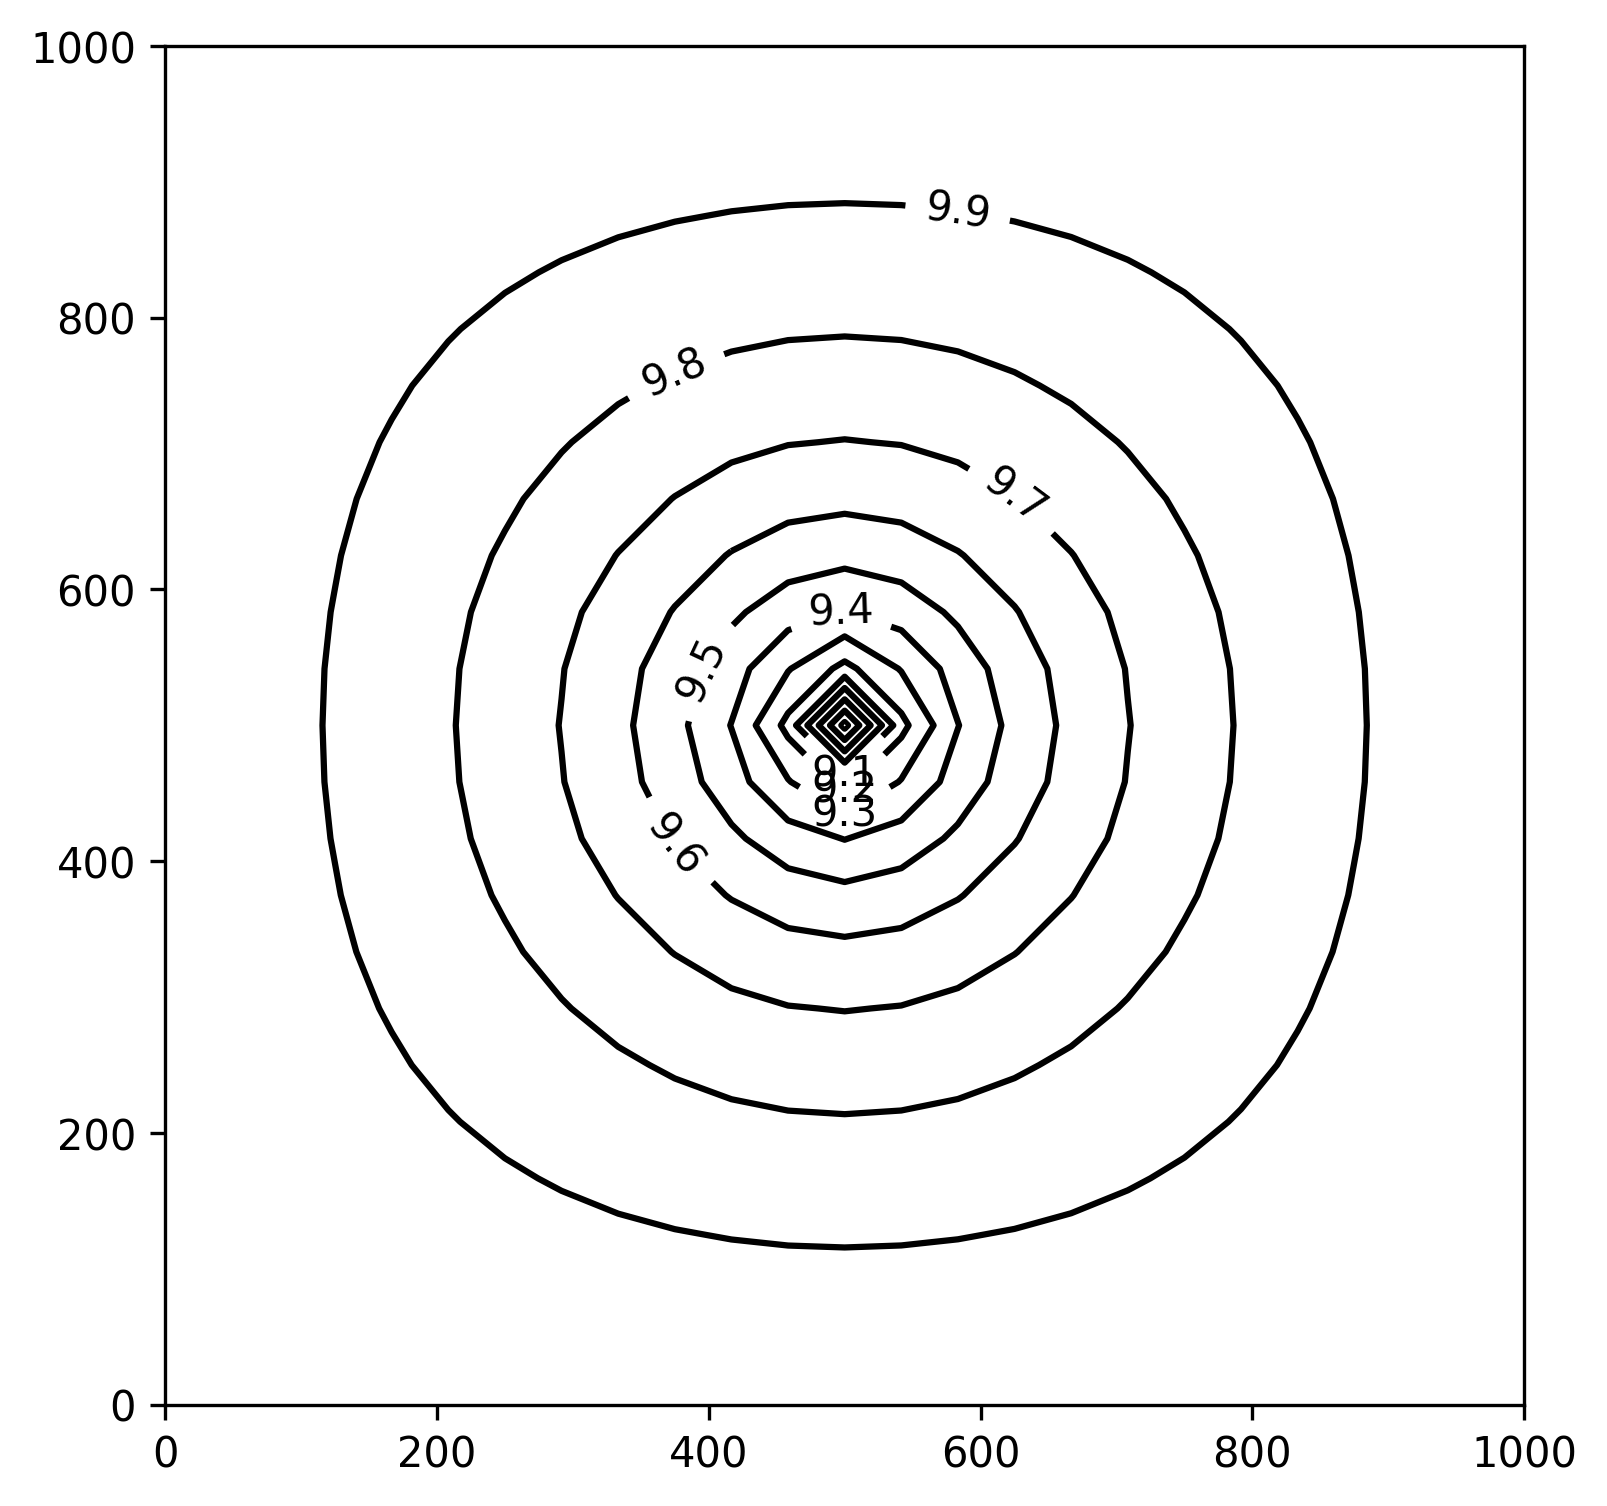
\includegraphics[width=0.7\textwidth]{Figures/appendix_figs/logbook1_heads_top.png}
\caption{top view of the hydraulic heads (m) in Model 1, with the x and y axis showing the lateral model dimensions (m).\label{fig_logbook1_top}}
\end{figure}

\begin{figure}[ht]
\centering
\includegraphics[width=1.0\textwidth]{Figures/appendix_figs/logbook1_heads_side.png}
\caption{Side view of the hydraulic heads (m) in all models and all layers. The side view shows row 12 out of 25 rows total (so approximately the centre row of the different models). The x axis shows the columns of the different models (also 25 total). Note that layer 1 always refers to the upper most layer, with deeper layers having increasingly higher numbers.\label{fig_logbook1_side}}
\end{figure}

